\section{Substitution genderbarer Textbestandteile}
\label{sec:substitution}
%Marcus

Als Kernfunktionalität der Software Equaly ist die Verarbeitung von eingegebenem Text zu gegendertem Text zu realisieren. Text muss dafür durch das Frontend aufgenommen und im Backend zumindest anteilig substituiert werden. Dazu wurde unter Verwendug der ausgewählten Technologien eine mit \ref{fig:pipeline} dargestellte KI-Pipeline entwickelt. Unverarbeiteter Text wird zunächst in seiner Gesamtheit an einen \textit{Language Detector} der Bibliothek Lingua\footnote{Die Bibliothek wurde über https://github.com/pemistahl/lingua bezogen.} weitergegeben. Dieser findet Verwendung, da er besonders wenig Text benötigt, um die verwendete Sprache bereits identifizieren zu können.

\begin{figure}[!th]
\centering
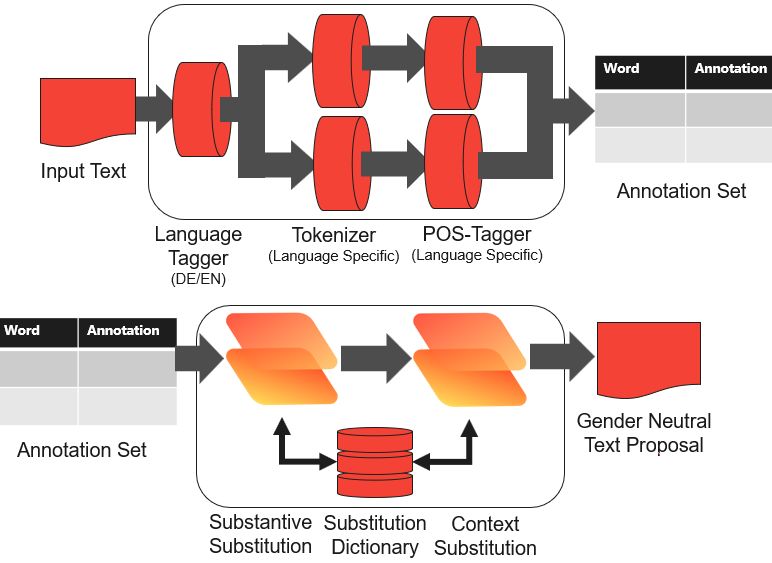
\includegraphics[width=9cm]{Resources/Pipeline.PNG}
\caption{Schematische Darstellung der KI-Pipeline}
\label{fig:pipeline}
\end{figure}

Abhängig von der erkannten Sprache, welche entweder Deutsch oder Englisch sein soll, wird anschließend ein Tokenizer-Modell der Bibliothek OpenNLP auf den Text angewendet. Die damit stattfindende Zerlegung in Sinnbausteine des Texts resultiert in einem Datensatz bestehend aus Token bzw. einzelnen Wortelementen. Diese Tokenmenge wird, erneut abhängig von der zuvor ermittelten Sprache, einem Part-of-Speech-Tagger (POS-Tagger) zugeführt. Der POS-Tagger wendet dabei ein vortrainiertes Maxent-Modell\footnote{Die verwendeten Modelle für Tokenizer und POS-Tagger wurden über http://opennlp.sourceforge.net/models-1.5/ bezogen.} an. Zwischenergebnis ist nun eine mit ihrer Sprache identifizierte Menge an Token, wobei die Token wie in \ref{fig:pos} zu sehen, durch den POS-Tagger mit Tags versehen wurden.

\begin{figure}[!th]
\centering
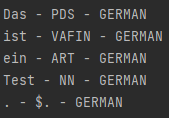
\includegraphics[width=2.5cm]{Resources/POS.PNG}
\caption{Ausgegebenes Zwischenergebnis der KI-Pipeline}
\label{fig:pos}
\end{figure}

Durch die angefügten Tags werden z.B. Substantive, irreflexible Personalpronomen und Eigennamen eindeutig voneinander differenzierbar. Auch Artikel sind nun als solche vermerkt, genau wie u.A. möglicherweise zu substituierende Demonstrativpronomen.

Um das Zeitbudget nicht zu überschreiten, wurde entschieden, Textvorschläge hauptsächlich durch Substitutionen genderbarer Substantive und ihnen zugehöriger Artikel zu erstellen. Aus dem Tokensatz werden diejenigen Token gefiltert, die mit einem Tag als Substantiv oder irreflexibles Personalpronomen versehen wurden. Dieses Subset wird gegen Einträge eines Dictionary in der SQLite-Datenbank geprüft. Sofern hier für ein Wort ein genderneutrales Substitut hinterlegt ist, wird dieses zurückgegeben und vermerkt. Zusätzlich werden Kasus, Numerus und Genus von vorherigem und neuem Wort aus dem Dictionary zurückgegeben und vermerkt.

Mit diesem Zwischenstand sind alle mit Dictionary-Einträgen erfassten Substantive und irreflexible Personalpronomen substituiert. Allerdings sind zugehörige Artikel nun ggf. mit dem falschen, alten Genus im Text vertreten. Um dieses Problem zu lösen wird der neue Tokensatz, sofern möglich, in seine einzelnen Sätze aufgeteilt. Pro Satz wird ermittelt, ob bereits ein Wort substituiert wurde. Ist dies der Fall, so werden mit dem dazu vermerkten Kasus, dem Numerus und dem Genus des alten Wortes alle im Satz vorhandenen Artikel, Relativpronomen und Demonstrativpronomen gefiltert. Sofern ein Wort hier eine Übereinstimmung mit altem Kasus, Numerus und Genus des bereits substituierten Wortes aufweist, muss es selbst ebenfalls substituiert werden. Dazu wird das Lemma des aktuellen, zu substituierenden Wortes im Dictionary gesucht. Mit diesem Lemma und altem Kasus, altem Numerus und neuem Genus wird dann ein Artikel der selben Wortfamilie, jedoch angepasst an das Subjekt- bzw. Objektsubstitut im Dictionary gesucht und im Text eingefügt. Beispielergebnisse dieses Substitutionsprozesses sind in \ref{fig:substitute} zu sehen.

\begin{figure}[!th]
\centering
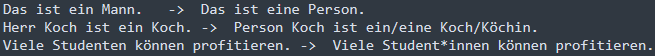
\includegraphics[width=9cm]{Resources/Substitution.PNG}
\caption{Beispielsätze und genderneutraler Substitutionsergebnisse}
\label{fig:substitute}
\end{figure}
